\section{Ondas II: Ondas Sonoras}
\subsection{Conteúdo Importante}
\subsubsection{Ondas Sonoras}
Uma onda sonora é uma onda longitudinal num meio elástico (e.g. gas, líquido ou sólido). Neste tipo de ondas, as partículas do meio oscilam para a frente e para trás ao longo da direção na qual a onda viaja, de onde resulta a criação de regiões de densidade alta e baixa. São estas regiões de compressão e rarefação que constituem as ondas que viajam pelo espaço e transportam energia.

\subsubsection{Velocidade do Som}
A velocidade do som varia com a propriedade elástica (que armazena energia potencial) e com a propriedade inercial (que armazena energia cinética) do meio onde se propaga. Uma expressão da forma geral para o som depende destes dois factores:

\begin{equation}\label{eq:ondas-v-geral}
    v=\sqrt{\frac{\text{properidade elástica}}{propriedade inercial}}
\end{equation}

Tomando como exemplo a Equação \ref{eq:onda-trans-v}, tem-se que a tensão $\tau$ na corda é a propriedade elástica da corda, enquanto que a densidade linear, $\mu$, é a propriedade inercial.

No caso de uma onda sonora que se propaga pelo ar, a propriedade elástica e propriedade inercial são a massa volúmica $\rho$ e o \emph{módulo de elasticidade volumétrico} $B$, respetivamente, onde $B$ é dado por:

\begin{equation}
    B=-\frac{\Delta p}{\Delta V/V}
\end{equation}

onde $\Delta V/V$ é a variação relativa de volume provocada pela variação $\Delta p$ de pressão. $B$ é sempre positivo tem unidades SI $Pa=1\ N\ m^{-2}$.

Por fim, a partir da Equação \ref{eq:ondas-v-geral}, temos a velocidade de propagação de uma onda sonora num meio com módulo de elasticidade $B$ e massa volúmica $\rho$:

\begin{equation}
    v=\sqrt{\frac{B}{\rho}}
\end{equation}

\subsubsection{Intensidade; Decibel}
A intensidade de uma onda, ou a potência por unidade de área, é a taxa à qual a energia que é transportada pela onda flui por unidade de área $A$ perpendicular à direção de propagação da onda. O ouvido humano pode detetar um intervalo grande de intensidades. Por esta razão, é conveniente usar uma escala logarítmica, onde o nível de som $\beta$ é definido pela equação

\begin{equation}
    \beta (dB)=10\log\frac{I}{I_0}
\end{equation}

onde $I_0$ é a intensidade de um nível de referência arbitrário considerado o "limear de audição" que é $I_0=1.0\cdot 10^{-12}Wm^{-2}$. A nível de exemplo, o nível de som de uma intensidade $I=1.0\cdot 10^{-5}Wm^{-2}$ será

\begin{equation}
    \beta=10\log\frac{1.0\cdot 10^{-5}Wm^{-2}}{1.0\cdot 10^{-12}Wm^{-2}}=10\log10^7=70\ dB
\end{equation}

\subsubsection{Batimentos}
Um fenómeno interessante que ocorre devido à interferência construtiva e destrutiva de duas ou mais frequências de som é o fenómeno dos \textbf{batimentos}. Se duas ondas diferirem em frequência, as ondas sonoras podem ser modeladas como

\begin{equation}
    y_1=A\cos(k_1x-2\pi f_1t) \qquad y_2=A\cos(k_2x-2\pi f_2t)
\end{equation}

Utilizando a identidade trigonométrica

\begin{equation}
    \cos u + \cos v=2\cos(\frac{u+v}{2})\cos (\frac{u-v}{2})
\end{equation}

e considerando $x=0.0m$, encontramos o som resultante num ponto do espaço, dado pela equação

\begin{equation}
    y(t; x=0\ m)=2A\cos(2\pi f_{media}t)\cos[2\pi(\frac{|f_2-f_1|}{2})t]
\end{equation}

onde a \textbf{frequência do batimento} é

\begin{equation}
    f_{batimento}=|f_2-f_1|
\end{equation}

\begin{figure}[h!]
    \centering
    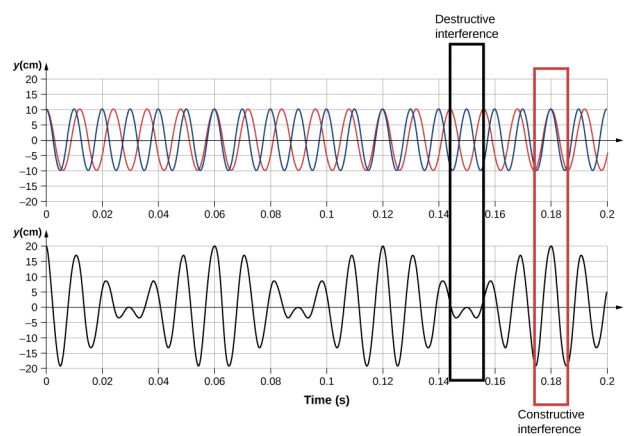
\includegraphics[width=0.5\textwidth]{12/fig/batimento.png}
    \caption{Batimento produzido pela interferência construtiva e destrutiva de duas ondas sonoras que diferem em frequência.}
\end{figure}
